\documentclass[a4paper, 11pt]{article}
\usepackage[margin=.5in]{geometry}
\usepackage{graphicx,amssymb,amstext,amsmath,amsthm,enumerate,float,textcomp}
\usepackage{pdfpages}
%\usepackage{listings}
\makeatletter
\renewcommand\@makefntext[1]{\leftskip=1em\hskip-2em\@makefnmark#1}
\makeatother

\begin{document}
\flushright
\begin{center}
\Large
STA 237  --- Time Series Analysis\\ Homework Series 1 \\ Rex Cheung  $\&$ Eliot Paisley \\ April 10, 2014 \\
\large  Prof. A.Aue \\ UC Davis
\end{center}

\flushleft 
\hrule \hrule 
\vspace{0.2in}
\begin{itemize}

	\item \textbf{Problem 1: [Stationarity]} Let $(Z_t: \; t \in \mathbb{Z})$ be a sequence of independent zero mean and normal random variables with variance $\sigma^2$ and let $a, b$, and $c$ be constants. Which of the following processess are weakly and/or strictly stationary? For wach weakly stationary process specify the mean and ACVF. 
	
	
	\begin{enumerate}[(a)]
		\item $X_t = a + bZ_t + cZ_{t-1}$. \newline 
		
			\underline{\emph{Answer:}} Let $i,j \in \mathbb{Z}$ be any two integers. Then, 
			$$E[X_i] = E[a + bZ_i + cZ_{i-1}] = a = E[a + bZ_j + cZ_{j-1}] = E[X_j],$$
			and
			$$Var[X_i] = Var[a + bZ_i + cZ_{i-1}] = 0 + b^2\sigma^2 + c^2\sigma^2 = Var[a + bZ_j + cZ_{j-1}] = Var[X_j], $$
where we have implicitly used the fact that every pair of $Z_t$ have zero covariance. \newline 

Thus, with knowledge that linear combinations of normally distributed random variables are normal, we have 
$$X_i,X_j \sim \mathcal{N}(a,(b^2+c^2)\sigma^2) .$$
Since $i,j$ were arbitrary, we have that every element $X_t$ has the same distribution, which implies that $X_t$ is \emph{strictly stationary}. \newline 

Since we have explicitly shown that we have finite variance, then we may also conclude that $X_t$ is \emph{weakly stationary}. $E[X_t] = a \; \forall t$, and note that 
$$Cov(X_{t+1},X_t) = Cov(a + bZ_{t+1} + cZ_{t}, a + bZ_t + cZ_{t-1} ) = Cov(cZ_t,bZ_t) = bc\sigma^2.  $$
Thus, 
$$\gamma(h) = \left\{\begin{array}{cc} (b^2+c^2)\sigma^2 & h = 0 \\ bc\sigma^2 & h=\pm 1 \\ 0 & |h|>1 \end{array}\right. .$$

		\item $X_t = Z_t\cos(ct) + Z_{t-1}\sin(ct)$ \newline 

			\underline{\emph{Answer:}} We will show that this is not stationary. First note that $E[X_t] = 0 \; \forall t$, and 
\begin{align*}			
Var[X_t] & = Var[Z_t\cos(ct) + Z_{t-1}\sin(ct)] \\
& = \sigma^2\cos^2(ct) + \sigma^2\sin^2(ct) = \sigma^2
\end{align*}
 and also
\begin{align*}
Cov(X_{t+1},X_t) & = Cov(Z_{t+1}\cos(ct+c) + Z_{t}\sin(ct+c),Z_t\cos(ct) + Z_{t-1}\sin(ct) ) \\
& = Cov(cZ_t,bZ_t) = \sin(ct+c)\cos(ct)\sigma^2
\end{align*}
Thus, 
$$\gamma(h) = \left\{\begin{array}{cc} \sigma^2 & h = 0 \\ \sin(ct+c)\cos(ct)\sigma^2 & h= + 1 \\ \cos(ct+c)\sin(ct)\sigma^2 & h= - 1 \\ 0 & |h|>1 \end{array}\right. .$$
The ACF depends on $t$, which violates the requirement that the ACF of a weakly stationary function is independent of $t$. Therefore, $X_t$ is not weakly stationary.\\

It is not strictly stationary either. Strictly stationary means the joint distribution is invariant under time shifts. If we take the random variables $(X_1, X_2)$ and $(X_3, X_4)$, we can see (from the calculation above) that they will have covariance that depends on $t$, which means the distribution is not the same. Thus $X_t$ is not strictly stationary.\newline 
			

		\item $X_t = a + bZ_0$ \newline 
		
			\underline{\emph{Answer:}} Let $i,j \in \mathbb{Z}$ be any two integers. Then, 
			$$E[X_i] = E[a + bZ_0] = a = E[a + bZ_0] = E[X_j],$$
			and
			$$Var[X_i] = Var[a + bZ_0] = 0 + b^2\sigma^2 = Var[a + bZ_0] = Var[X_j].$$

Thus, with knowledge that linear combinations of normally distributed random variables are normal, we have 
$$X_i,X_j \sim \mathcal{N}(0,b^2\sigma^2) .$$
Since $i,j$ were arbitrary, we have that every element $X_t$ has the same distribution, which implies that $X_t$ is \emph{strictly stationary}. \newline 

Since we have explicitly shown that we have finite variance, then we may also conclude that $X_t$ is \emph{weakly stationary}. $E[X_t] = 0 \; \forall t$, and 
$$\gamma(h) = b^2\sigma^2, \forall h. $$

		\item $X_t = Z_tZ_{t-1}$ \newline 
		
			\underline{\emph{Answer:}} We will first show that this is weakly stationary, and then strictly stationary. First note that $\forall t$, 
\[ E[X_t] = E[Z_tZ_{t-1}] = E[Z_t]E[Z_{t-1}] = 0\]
\[ E[X_t^2] = E[Z_t^2Z_{t-1}^2] = \sigma_{tt}\sigma_{(t-1),(t-1)} + \sigma_{t,t-1}\sigma_{t,t-1} + \sigma_{t,t-1}\sigma_{t,t-1} = \sigma^4  \]
where $\sigma_{ij}$ is the covariance between the $i^{th}$ and $j^{th}$ random variable. To compute the ACF, we apply the same idea: $\forall h$ such that $t+h \in T$, 
\begin{align*}
cov(X_{t+h}, X_t) &= cov(Z_{t+1}Z_{t-1+h}, Z_tZ_{t-1}) \\
&= E[Z_{t+1}Z_{t-1+h}Z_tZ_{t-1}] - E[Z_{t+1}Z_{t-1+h}]E[Z_tZ_{t-1}] \\
&= 0 \quad \text{ if $h \neq 0$}
\end{align*}
Thus, 
$$\gamma(h) = \left\{\begin{array}{cc} \sigma^4 & h = 0 \\  0 & |h|>1 \end{array}\right. .$$
			To show this is strictly stationary, first note that
\[(Z_t, Z_{t+1}, ..., Z_{t+k}) \approx^{\mathcal{D}} (Z_{t+h}, Z_{t+1+h}, ..., Z_{t+k+h})\] \\
In fact, we can use any index set $T$ and will get the same result. Now just treat $(X_t, X_{t+1}, ..., X_{t+k})$ as a functional transformation of $(Z_t, Z_{t+1}, ..., Z_{t+k})$, i.e.$(X_t, X_{t+1}, ..., X_{t+k}) = g(Z_t, Z_{t+1}, ..., Z_{t+k})$, which still have identical distribution as $g(Z_{t+h}, Z_{t+1+h}, ..., Z_{t+k+h})$.

	\end{enumerate}
	
	
	\hrule 
	\newpage 
	\item \textbf{Problem 2: [U.S. Population]} Download the file \texttt{population.xls} from the course website. It contains the size of the population in the U.S.A. at ten-year intervals from 1790 to 2000. 
	
	
	\begin{enumerate}[(a)]
		\item Plot the data. \newline 
		
		\emph{See Figure 1.}
\begin{figure}
\centering
\begin{minipage}{.5\textwidth}
  \centering
	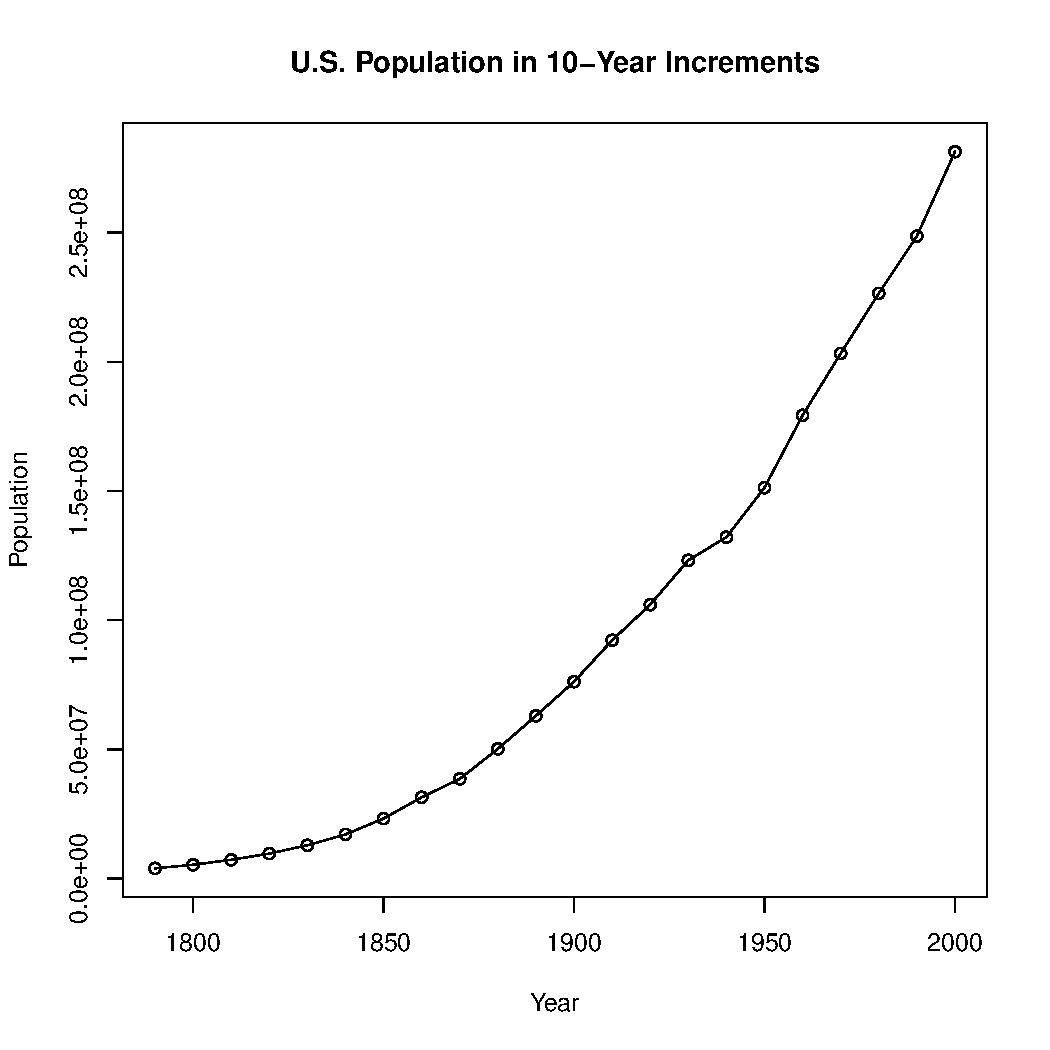
\includegraphics[scale=0.5]{hw1_dataplot.pdf}
  \caption{Plot of the population data for Problem 2}
\end{minipage}%
\begin{minipage}{.5\textwidth}
  \centering
  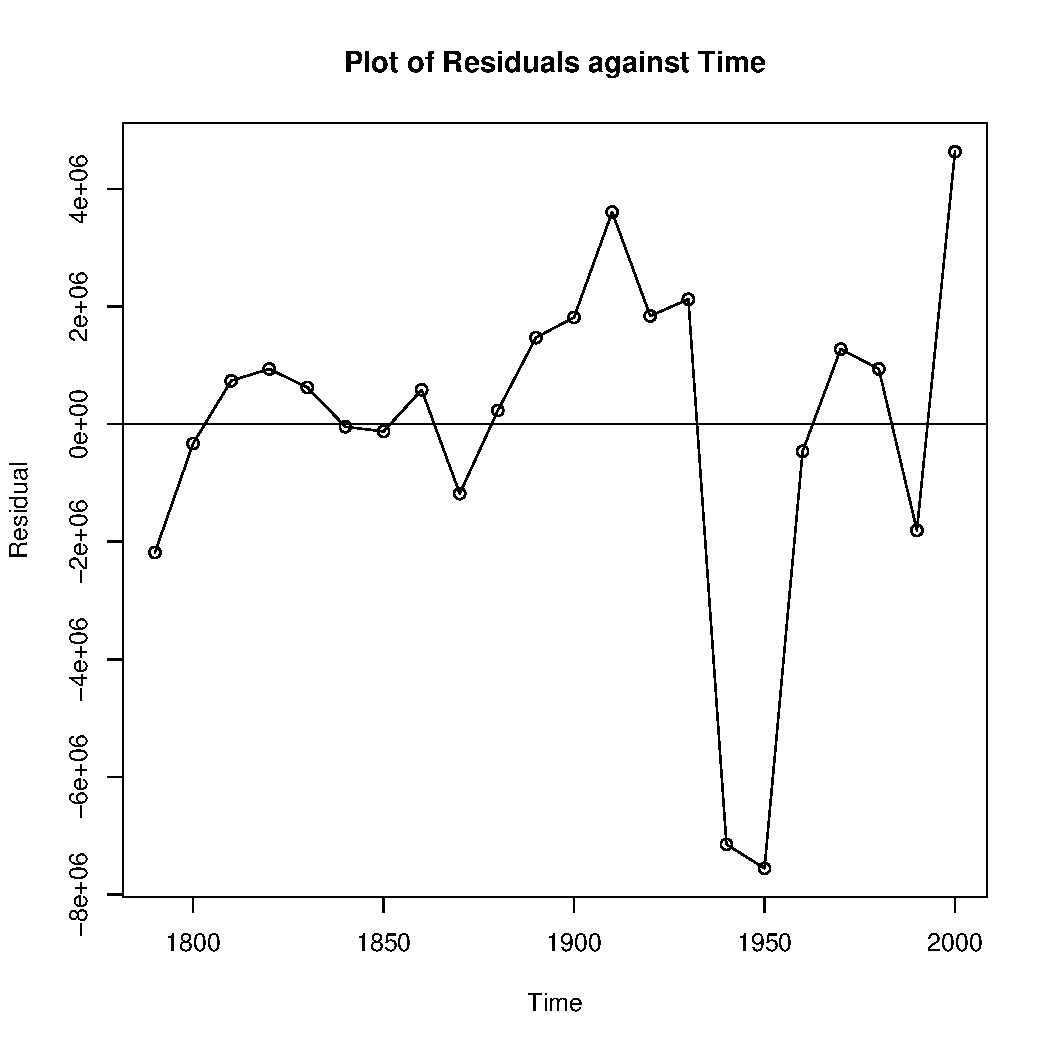
\includegraphics[scale=0.5]{hw1_resid.pdf}
  \caption{Plot of the Residuals against Time for the fitted values in Table 1.}
\end{minipage}
\end{figure}

		\item Assuming the model $X_t = m_t + Z_t$, $E[Z_t] = 0$, fit a polynomial trend $\widehat{m}_t$ to the data. \newline 
		
		\emph{See Table 1 for the fitted values for a $2^{nd}$ degree polynomial}
		
\begin{table}[h!]
\small
\centering
\begin{tabular}{r}
  \hline
	$\widehat{m}_t$\\ 
  \hline
	6110720.45 \\ 
  5637937.68 \\ 
  6501266.64 \\ 
  8700707.34 \\ 
  12236259.78 \\ 
  17107923.95 \\ 
  23315699.86 \\ 
  30859587.50 \\ 
  39739586.88 \\ 
  49955698.00 \\ 
  61507920.85 \\ 
  74396255.44 \\ 
  88620701.76 \\ 
  104181259.82 \\ 
  121077929.62 \\ 
  139310711.15 \\ 
  158879604.42 \\ 
  179784609.42 \\ 
  202025726.16 \\ 
  225602954.63 \\ 
  250516294.84 \\ 
  276765746.79 \\ 
   \hline
\end{tabular}
\caption{Fitted values for a $2^{nd}$ degree polynomial fit}
\end{table}

		\item Plot the residuals $\hat{Z}_t = X_t - \hat{m}_t$. Comment on the quality of the fitted model. \newline 

		\emph{See Figure 2.} This residual plot shows a bit of structure, but not too much where we would have considerable worry regarding the model fit. 
		\item Use the fitted model to predict the population size in 2010 and 2020 (using predicted noise values of zero). \newline 
		
		\emph{See Table 2.}
		
		\begin{table}[h!]
		\centering
		\begin{tabular}{rrr}
			\hline
			& 2010 & 2020 \\ 
			\hline
		$\widehat{m}$ & 304351310.47 & 333272985.89 \\ 
			\hline
		\end{tabular}
		\caption{Predicted population values for the years 2010 and 2020.}
		\end{table}

\begin{verbatim}
########
# R Code
########
rm(list=ls(all=TRUE))
library(xtable)
library(matrixcalc)
setwd("C:/Users/EliotP/Documents/GitHub/STA_237_sp14/Homework/") #laptop
pop = as.matrix(read.table("population.csv"))
n = nrow(pop)

### plot the data
time = as.vector(seq(1790,2000,10))
pdf("hw1_dataplot.pdf")
plot(time,t(pop),type="o",xlab="Year",
			ylab="Population",main="U.S. Population in 10-Year Increments")
dev.off()

### fit a 2nd degree polynomial
F = vandermonde.matrix(1:n,3)
mhat_ls = F%*%solve(t(F)%*%F)%*%t(F)%*%pop 

print(xtable(mhat_ls),include.rownames=FALSE)

### residuals

resid = pop-mhat_ls
pdf("hw1_resid.pdf")
plot(x=time, resid,type="o",xlab="Time",
			ylab="Residual",main="Plot of Residuals against Time")
abline(h=0)
dev.off()

### predict using direct method
A=solve(t(F)%*%F)%*%t(F)%*%pop
predict_val = as.matrix(c(A[1]*1+A[2]*23+A[3]*23^2,A[1]*1+A[2]*24+A[3]*24^2))
print(xtable(t(predict_val)),include.rownames=FALSE)
\end{verbatim}
\end{enumerate}
	

	\hrule 
	\newpage \newpage 
	\item \textbf{Problem 3: [Projection Theorem]} If $\mathcal{M}$ is a closed subspace of a Hilbert Space $\mathcal{H}$ and $x\in\mathcal{H}$, prove that 
	$$\underset{y\in\mathcal{M}}{\min}||x-y|| = \max\left\{|\langle x,z\rangle|: z\in \mathcal{M}^\bot, ||z|| = 1  \right\} ,$$
where $\mathcal{M}^\bot$ is the orthogonal complement of $\mathcal{M}$. \newline 

	\underline{\emph{Answer:}}
	
Begin by writing $x = x_1 + x_2$, with $x_1 \in \mathcal{M}, x_2\in\mathcal{M}^\bot$, which is allowed by the orthogonal decomposition theorem \footnote{http://en.wikibooks.org/wiki/Functional$\_$Analysis/Hilbert$\_$spaces, section 3.6}.

	Now, consider
	$$||x-y||^2 = ||x_1+x_2 - y||^2 = \langle x_1+x_2-y, x_1+x_2-y\rangle = \langle x_1-y+x_2, x_1-y+x_2\rangle = ||x_1-y||^2 + ||x_2||^2. $$
	Hence, 
	$$ \underset{y\in\mathcal{M}}{\min}||x-y|| = \underset{y\in\mathcal{M}}{\min}||x_1-y||^2 + ||x_2||^2 = ||x_2||^2,$$
	where the minimum is achieved at $y = x_1\in\mathcal{M}$. \newline 
	
	On the other hand, for any $z\in \mathcal{M}^\bot, ||z||=1$,  
	$$|\langle x,z \rangle | = |\langle x_1+x_2,z \rangle | = |\langle x_1,z \rangle +\langle x_2,z \rangle | = |\langle x_2,z \rangle |,  $$
	and 
	$$|\langle x_2,z \rangle |\leq ||x_2|| ||z|| = ||x_2|| $$
	by the Cauchy-Schwartz inequality. This implies that 
	$$|\langle x,z \rangle | \leq ||x_2||. $$
		It follows that 
	$$\max\left\{|\langle x,z\rangle|: z\in \mathcal{M}^\bot, ||z|| = 1  \right\} = ||x_2||,$$
	where the maximum is achieved at $z = \frac{x_2}{||x_2||}$. \newline 
	Thus, 
	$$\underset{y\in\mathcal{M}}{\min}||x-y|| = ||x_2|| = \max\left\{|\langle x,z\rangle|: z\in \mathcal{M}^\bot, ||z|| = 1  \right\} ,$$
		%\hrule 
	%We show the desired result in two cases:\newline
	%
	%Case 1: Suppose that $x\in\mathcal{M}$. Then $\underset{y\in\mathcal{M}}{\min}||x-y|| = 0$, where the minimum is obtained at $y = x$. Moreover, $\langle x,z\rangle = 0\; \forall z\in \mathcal{M}^\bot$, due to orthogonality. \newline 
	%
	%Case 2: Suppose that $x\in\mathcal{M}^\bot$. Then, for $y\in\mathcal{M}, z\in\mathcal{M}^\bot$,  we can write 
	%$$\langle x,z \rangle = \langle x-y,z \rangle + \langle y,z\rangle  = \langle x-y,z \rangle,$$
	%and by the triangle inequality,
	%$$\langle x-y,z \rangle \leq ||x-y|| ||z|| = ||x-y||.$$
	%Thus, we have 
	%$$\langle x,z \rangle \leq ||x-y||,$$
	%and it follows naturally that in order for equality to hold we must have the maximum on the left-hand-side, and the minimum on the right-hand-side. That is, 
	%$$\max \langle x,z \rangle  = \min ||x-y||.$$
	%
	\hrule 
	\item \textbf{Problem 4: [Prediction Equations]} If $X_t = Z_t - \theta Z_{t-1}$, where $|\theta| <1$ and $(Z_t: t\in\mathbb{Z})$ is a sequence of uncorrelated random variables, each with mean 0 and variance $\sigma^2$, show by checking the prediction equations that the best mean square predictor of $X_{n+1}$ in $\overline{\text{sp}}(X_j: j \leq n)$ is 
	$$\hat{X}_{n+1} = -\sum_{j=1}^\infty \theta^j X_{n+1-j}. $$
	What is the mean squared error of $\hat{X}_{n+1}$?

	\underline{\emph{Answer:}} To show that $\hat{X}_{n+1} = -\sum^{\infty}_{j=1}\theta^jX_{n+1-j}$ is the best mean square predictor of $X_{n+1}$, we need to show this predictor satisfies the prediction equations, i.e. 
\[ \langle X_{n+1} - \hat{X}_{n+1}, X_j \rangle = 0 \quad \quad \forall j \leq n\]
First rewrite $X_{n+1}$ as the following:
\begin{align*}
X_{n+1} = Z_{n+1} - \theta Z_n &= Z_{n+1} - \theta(X_n + \theta Z_{n-1}) \\
&= Z_{n+1} - \theta X_n - \theta^2 Z_{n-1} \\
&= Z_{n+1} - \theta X_n - \theta^2(X_{n-1} + \theta Z_{n-2}) \\
&= Z_{n+1} - \theta X_n - \theta^2 X_{n-1} - \theta^3 Z_{n-2}\\
&= \vdots \\
&= Z_{n+1} - \sum^{\infty}_{j=1}\theta^jX_{n+1-j}
\end{align*}
Then the prediction equation simplifies to
\[ <X_{n+1} - \hat{X}_{n+1}, X_j>  = <Z_{n+1},X_j> = E[Z_{n+1}X_j] \quad \quad \forall j \leq n \]
Rewriting $E[Z_{n+1}X_j]$ as $E[Z_{n+1}(Z_j - \theta Z_{j-1})]$, we can see this expectation is 0 $\forall j \leq n$ because of independence. Thus $\hat{X}_{n+1}$ satisfies the condition to be the best mean square predictor of $X_{n+1}$. \\
The mean squared error of $\hat{X}_{n+1}$ is then
\[
E[|X_{n+1} - \hat{X}_{n+1}|^2] = E[|Z_{n+1}|^2] = \sigma^2
\]
	
	\hrule 


\end{itemize}	
\end{document}












